\bookchapter{Bab 60: Menyiapkan persekitaran pembangunan — Xcode dan projek pertama}

\chapterintro{Untuk kerja yang baik, pertajam dahulu alatnya. Dalam bab ini kita “menyiapkan dapur”: memasang Xcode, memastikan simulator berjalan, mencipta projek iOS pertama dalam hidup anda, kemudian mengurai struktur projek sehingga jelas. Selepas persekitaran siap, anda akan buat pertama kali melihat kod yang anda tulis menjadi butang yang boleh ditekan — detik ini, ramai orang ingat seumur hidup.}

\booksection{Sediakan sebuah Mac}

Syarat dahulu: pembangunan iOS mesti dilakukan pada macOS. Jika anda tidak mempunyai Mac, ada tiga pilihan: beli satu (walaupun Mac mini atau MacBook Air terpakai pun cukup), sewa Mac awan untuk jangka pendek, atau baca dahulu Bahagian 8 “Amalan Pembangunan Android” (boleh dilakukan pada Windows).

\begin{center}
\begin{tabularx}{\linewidth}{|X|X|X|}
\hline
\textbf{Perkara konfigurasi} & \textbf{Keperluan minimum} & \textbf{Tahap selesa (disyorkan)} \tabularnewline
\hline
Cip & Apple Silicon (M1 ke atas) & M2 atau lebih baharu \tabularnewline
Memori & 8GB & 16GB \tabularnewline
Cakera & Ruang 40GB+ (Xcode sendiri sangat besar) & Bermula 256GB \tabularnewline
Sistem & macOS terkini & Kekalkan kemas kini automatik \tabularnewline
\hline
\end{tabularx}
\end{center}

\begin{center}\small\color{gray}Rujukan konfigurasi mesin pembangunan Mac (Ogos 2026)\end{center}

\begin{tcbinfo}{Petua: boleh belajar bahasa dahulu walaupun tiada Mac}
Swift Playgrounds yang percuma di iPad boleh mengajar asas bahasa Swift (tanpa Mac); malah boleh dipasang di iPhone juga. Kuasai dahulu pengetahuan bahasa Bab 61 dalam Playgrounds; apabila mendapat Mac, anda terus meluncur. “Mengasah kapak tidak melambatkan menebang kayu” — itulah maksudnya.

\end{tcbinfo}

\booksection{Memasang Xcode}

Xcode ialah persekitaran pembangunan bersepadu rasmi Apple, percuma. Tiga langkah untuk memasang:

\begin{enumerate}
  \item Di Mac, buka App Store, cari "Xcode", tekan pasang — ingat, saiznya beberapa GB, pilih waktu yang rangkaiannya laju;
  \item Selepas terpasang, lancarkan buat kali pertama, setuju dengan perjanjian dan biar komponen selesai dipasang (berlaku secara automatik);
  \item Menu Xcode Settings Locations, pastikan Command Line Tools telah dipilih — alat baris arahan ialah prasyarat bagi banyak skrip dan alat pihak ketiga.
\end{enumerate}

\begin{tcbwarn}{Perhatian: "permainan padanan" antara versi dan sistem}
Xcode baharu kerap menuntut macOS terkini, manakala Mac lama akan terkandas pada versi lama. Semasa menerbitkan ke App Store, Apple menuntut binaan dengan Xcode yang lebih baharu (biasanya diberikan tempoh tangguh). Jadi jangan tangguh kemas kini sistem terlalu lama — pembangun iOS antara kumpulan yang paling rajin mengejar versi baharu.

\end{tcbwarn}

\booksection{Mencipta projek pertama anda}

Buka Xcode Create New Project pilih iOS templat App, kemudian isi:

\begin{center}
\begin{tabularx}{\linewidth}{|X|X|X|}
\hline
\textbf{Perkara konfigurasi} & \textbf{Apa yang diisi} & \textbf{Penjelasan} \tabularnewline
\hline
Product Name & MyFirstApp & Nama aplikasi \tabularnewline
Team & Apple ID anda (percuma) & Untuk tandatangan, akaun peribadi sudah cukup \tabularnewline
Organization Identifier & com.example & Digabung dengan Product Name menjadi pengenal pakej \tabularnewline
Interface & SwiftUI & Rangka kerja garis utama buku ini \tabularnewline
Language & Swift & Tak perlu dijelaskan \tabularnewline
\hline
\end{tabularx}
\end{center}

\begin{center}\small\color{gray}Lima perkara yang diisi semasa mencipta projek\end{center}

Selepas menekan Create, Xcode akan menjana projek yang boleh terus dijalankan. Pilih satu simulator di penjuru kiri atas (contohnya iPhone 17), tekan > untuk menjalankan — beberapa saat kemudian, di skrin simulator muncul satu tetingkap bertulis “Hello, world!”. Aplikasi iOS pertama anda telah dilahirkan.

\booksection{Mengurai struktur projek: apa fungsi setiap fail}

Di sebelah kiri ialah navigator projek; pemula hanya perlu mengenali beberapa ini:

\begin{center}
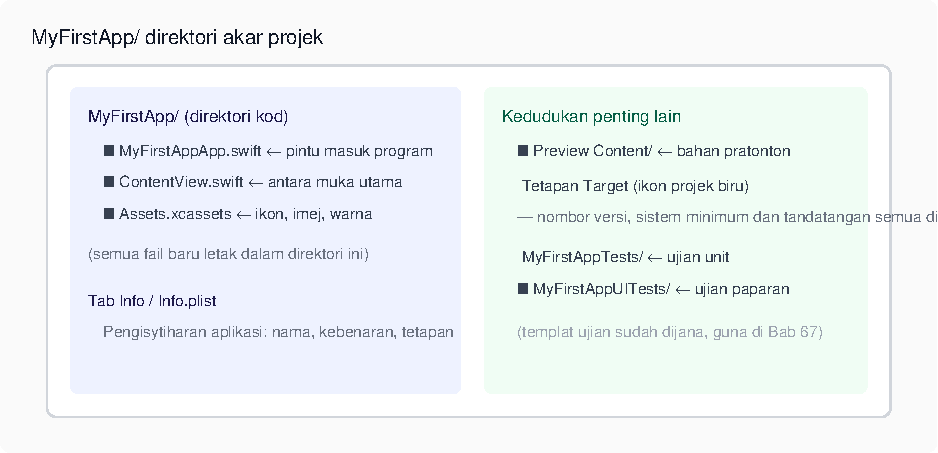
\includegraphics[width=0.92\linewidth]{figures/fig-di-liu-shi-zhang-1}
\\[2pt]\small Rajah 2: Struktur projek Xcode yang wajib difahami pemula
\end{center}

\begin{itemize}
  \item MyFirstAppApp.swift: pintu masuk program; dalam SwiftUI ia hanya beberapa baris — "mula, kemudian paparkan antara muka utama";
  \item ContentView.swift: paparan antara muka utama; semua yang anda lihat sekarang ada di sini;
  \item Assets.xcassets: gudang sumber — ikon, imej dan warna diletakkan di sini;
  \item Tetapan Target: tekan ikon projek biru di sebelah kiri untuk masuk; nombor versi, versi iOS minimum dan tandatangan semuanya di dalamnya. Nama paparan aplikasi dan ikon juga dikonfigur di sini.
\end{itemize}

\booksection{Debug pada peranti sebenar: memasang aplikasi ke dalam iPhone anda}

\booksection{Petua kecekapan Xcode: lima “senjata rahsia pintasan” pemula}

Kuasai yang berikut, dan anda akan kelihatan “sangat profesional”:

\begin{center}
\begin{tabularx}{\linewidth}{|X|X|X|}
\hline
\textbf{Tindakan} & \textbf{Pintasan} & \textbf{Fungsi} \tabularnewline
\hline
Menjalankan & CmdR & Kompil dan jalankan \tabularnewline
Buka/tukar pratonton kanvas & OptionCmd & Suis "apa yang dilihat itulah yang diperoleh" \tabularnewline
Format inden & CtrlI & Menyusun inden kod yang dipilih secara automatik \tabularnewline
Buka fail dengan pantas & CmdO & Taip nama fail, terbuka serta-merta (paling kerap digunakan!) \tabularnewline
Komen/nyahkomen & Cmd/ & Hidup/matikan kod dengan pantas semasa debug \tabularnewline
\hline
\end{tabularx}
\end{center}

\begin{center}\small\color{gray}Pintasan papan kekunci Xcode yang kerap digunakan (lima serangkai pemula)\end{center}

Dua faedah tersembunyi lagi: menjalankan beberapa simulator serentak (jalankan iPhone dan iPad pada masa yang sama untuk membandingkan susun atur) dan pustaka petikan kod (seret beberapa baris kod biasa ke panel Snippets di sebelah kanan, lain kali sisipkan dengan satu tekanan) — gunakan dahulu alat kecekapan ini, dan kemahiran tangan akan datang dengan sendirinya.

\booksection{Debug pada peranti sebenar: memasang aplikasi ke dalam iPhone anda}

Walaupun simulator bagus, peranti sebenar tetap destinasi akhir. Dengan Apple ID percuma pun boleh debug pada peranti sebenar:

\begin{enumerate}
  \item Sambungkan iPhone dengan kabel data (atau debug secara wayarles melalui Wi-Fi yang sama);
  \item Dalam senarai peranti di bahagian atas Xcode, pilih telefon anda; kali pertama akan diminta log masuk Apple ID dan tandatangan dikonfigur secara automatik;
  \item Di iPhone, [Tetapan] [Am] [VPN \& Pengurusan Peranti] percayai sijil pembangun anda;
  \item Tekan >, dan aplikasi terpasang pada peranti sebenar.
\end{enumerate}

\begin{tcbwarn}{Perhatian: "had tujuh hari" akaun percuma}
Aplikasi yang ditandatangani dengan Apple ID percuma akan luput selepas 7 hari (jalankan semula sekali untuk memperbaharui). Ini mekanisme cegah penyalahgunaan Apple; untuk peringkat pembelajaran ia sudah cukup; akaun pembangun berbayar (99 dolar AS setahun) tiada had ini, diterangkan terperinci dalam Bab 67.

\end{tcbwarn}

\booksection{Ujian kemahiran pertama + pertolongan cemas ralat biasa}

\booksection{Ujian kemahiran pertama + pertolongan cemas ralat biasa}

Buka ContentView.swift, tukar teks dalam Text(“Hello, world!”) kepada nama anda, tekan CmdR untuk menjalankan semula — beberapa saat kemudian nama anda dipaparkan pada simulator. Tahniah, anda telah menamatkan pusingan penuh pertama “ubah kod kompil pasang jalankan”.

\begin{center}
\begin{tabularx}{\linewidth}{|X|X|X|}
\hline
\textbf{Gejala ralat} & \textbf{Punca biasa} & \textbf{Penawar} \tabularnewline
\hline
Ralat Signing & Team tidak dipilih, sijil luput & Dalam Target Signing, tandakan akaun anda; untuk akaun percuma, jalankan semula sekali \tabularnewline
Skrin simulator hitam/tidak boleh dibuka & Imej rosak & Menu Device Erase All Content; atau padam dan tambah semula simulator \tabularnewline
Muat turun Xcode perlahan/gagal dipasang & Rangkaian App Store tidak stabil & Tukar waktu; atau muat turun pakej luar talian .xip dari laman pembangun Apple \tabularnewline
\hline
\end{tabularx}
\end{center}

\begin{center}\small\color{gray}Jadual pertolongan cemas ralat persekitaran untuk pemula\end{center}

\begin{tcbpractice}{Praktik: lengkapkan senarai "ritual pembangunan" anda}
(1) Pasang Xcode dan pastikan simulator berjalan; (2) jalankan aplikasi anda sekali pada peranti sebenar dan simpan tangkapan skrin sebagai kenangan; (3) tukar teks Hello kepada nama anda; (4) dalam tetapan Target, tukar nama paparan aplikasi kepada “Aplikasi Pertama Saya”. Selepas empat langkah ini, anda sudah ialah orang yang berkarya.

\end{tcbpractice}

\begin{tcbsummary}{Ringkasan bab ini}
\begin{itemize}
  \item Syarat wajib: Mac + Xcode; tiada Mac? Belajar bahasa dahulu dengan Swift Playgrounds di iPad
  \item Xcode dipasang dari App Store; versi baharu menuntut sistem baharu, jangan tangguh kemas kini
  \item Lima unsur projek baharu: nama, Team, pengenal organisasi, SwiftUI, Swift
  \item Petua projek: semua kod dalam direktori MyFirstApp/; tetapan Target mengurus versi dan tandatangan
  \item Debug peranti sebenar dengan Apple ID percuma ada had tandatangan 7 hari; akaun berbayar tiada had ini
  \item Rutinan pembangunan = ubah kod CmdR lihat hasil, berulang-ulang
\end{itemize}

\end{tcbsummary}
